\documentclass{scrartcl}
\usepackage{amsmath, amssymb}
\usepackage{graphicx, float}
\usepackage{hyperref}
\usepackage[T1]{fontenc}
\begin{document}
\begin{center}
\textbf{\LARGE ACE Documentation}\\[2mm]
\textit{\Large Moritz Cygorek}
\end{center}
\section{Introduction}
This document is intended to describe how to use the C++ code ACE
for the solution of open quantum systems using the 
\emph{automated compression of environments} (ACE) method.
The article explaining the method can be found 
\href{https://arxiv.org/abs/2101.01653}{here}.

Generally, ACE provides numerically exact simulation of the dynamics of 
an open quantum systems described by the microscopic Hamiltonian 
%\begin{align}
\begin{equation}
H=H_S+H_E = H_S +\sum_{k=1}^{N_E} H_E^k,
\end{equation}
%\end{align}
where $H_S$ is the system Hamiltonian and the environment Hamiltonian $H_E$,
which also includes the system-environment coupling, is assumed to be 
separable into $N_E$ independent modes $k$. 
Throughout this document we will denote the dimension of the system Hilbert
space by $N$ while the dimension of the $k$-th environment mode
is $M^k$ (or simply $M$ if all $M^k$ are identical).

The goal is to obtain the reduced system density matrix discretized on
a time grid $t_l = t_a + l \Delta t$ up to a given final time 
$t_n = t_a + n \Delta t = t_e$.
This can be done using the path integral expression
\begin{equation}
{\rho}_{\alpha_n}=
\sum_{\substack{\alpha_{n-1}\dots\alpha_0 \\
\tilde{\alpha}_n\dots\tilde{\alpha}_1}}
\mathcal{I}^{(\alpha_{n}\tilde{\alpha}_n)\dots(\alpha_1\tilde{\alpha}_1)}
\bigg(\prod_{l=1}^{n}
\mathcal{M}^{\tilde{\alpha}_{l}\alpha_{l-1}} \bigg)
{\rho}_{\alpha_0},
\end{equation}
where ${\rho}_{\alpha_l}={\rho}_{\nu_l \mu_l}$ is the reduced 
system density matrix at time step $l$, $\mathcal{M}$ describes the
free time evolution of the system, and $\mathcal{I}$ is the 
\emph{process tensor} (PT) accounting for the 
effects of the environment.
To keep the notation compact, we combine two Hilbert space indices
on the system density matrix $\nu_l$ and $\mu_l$ into a single 
Liouville space index $\alpha_l=(\nu_l, \mu_l)$.
The GIF can always expressed in the form of a matrix product operator (MPO)
%
\begin{equation}
\mathcal{I}^{(\alpha_{n},\tilde{\alpha}_{n})(\alpha_{n-1},\tilde{\alpha}_{n-1})
\dots (\alpha_{1},\tilde{\alpha}_{1})}
= 
\sum_{d_{n-1}\dots d_1}
\mathcal{Q}_{1 d_{n-1}}^{(\alpha_{n},\tilde{\alpha}_{n})}
\mathcal{Q}_{d_{n-1} d_{n-2}}^{(\alpha_{n-1},\tilde{\alpha}_{n-1})}\dots
\mathcal{Q}_{d_1 1}^{(\alpha_{1},\tilde{\alpha}_{1})}.
\end{equation}
In the explicit derivation of the matrices $\mathcal{Q}$, the inner indices
$d_l$ correspond to a complete basis of the Liouville space 
of the full environment, which can be extremely large. However, the inner 
dimensions of MPOs can be systemaically reduced using established compression 
techniques.
Here, we use a compression method based on singular value decomposition (SVD),
where singular values below a predefined threshold $\epsilon$ are disregarded.
The time discretization $\Delta t$ and the compression threshold $\epsilon$
are the main convergence parameters of ACE.

The working principle of ACE is to construct the PT in compressed MPO form
by calculating the PTs for the individual environment modes $k$ 
and then combining them one by one. 
After each combination step, the GIF MPO is compressed using
SVDs to reduce the inner dimensions to a manageable size at all times.
Once the compressed PT is calculated,
the reduced system density matrix for a given 
system Hamiltonian and system initial state can be obtained by contracting
a simple tensor network.

\section{Code, Compilation, Dependencies, and Design Choices}
The code has been written in C++ to combine low-level optimization 
(memory storage, access to LAPACK routines) with high-level abstraction
for better usability. Although nothing in the code depends explicitly on the
operating system, the code has been tested only on Linux.

We have tried to keep the dependencies on other codes minimal.
However, the \href{http://eigen.tuxfamily.org}{Eigen} library is very handy
and provides useful and efficient routines, e.g., for matrix exponentials.
We use it in particular to specify Hamiltonians and density matrices.
The numerically most demanding part of ACE is the calculation of SVDs. 
Here, we make use of the corresponding LAPACK routines. In my experience, the 
\href{https://software.intel.com/content/www/us/en/develop/tools/math-kernel-library.html}{Intel MKL} 
implementation of the SVD LAPACK routines can be significantly faster than
other implementations, sometimes by orders of magnitudes.
Therefore, we assume that Eigen as well as the Intel MKL is installed on the
computer. 

The installation of ACE via Makefiles needs to be able to find 
these libraries. To this end, the corresponding Linux environment variables 
have to be set.
A successful installation of MKL should automatically set the 
\texttt{MKLROOT} environment variable to the correct directory.
We assume that the Eigen library is installed in the directory
\texttt{/usr/include/eigen3/}. If not, please set the variable 
\texttt{EIGEN\_HOME} manually in such a way that the file 
\texttt{\$EIGEN\_HOME/Eigen/Eigen} exists.

To compile the code, go into the main directory of ACE and type in the
console
\begin{verbatim}
> make 
\end{verbatim}
This should compile the code and copy the binaries into the \texttt{bin/}
subdirectory. For easy access later on, we suggest to add this directory
to your Linux environment via the \texttt{PATH} variable. For example, 
add the follwing line to your \texttt{$\sim$/.bashrc} file 
\begin{verbatim}
PATH=/.../ACE/bin/:$PATH 
\end{verbatim}
where the $\dots$ are to be replaced to point to the correct absolute directory.
Log out and log in again to activate the changes. Then, go to a temporary
directory and run
\begin{verbatim}
> ACE
\end{verbatim}
This should generate a file \texttt{ACE.out} whose first lines are
\begin{verbatim}
0 0 0 1 0 0 0 inf inf
0.01 0 0 1 0 0 0 1 0
0.02 0 0 1 0 0 0 1 0
0.03 0 0 1 0 0 0 1 0
0.04 0 0 1 0 0 0 1 0
...
\end{verbatim}
Congratulations! You have just executed your first (rather boring) simulation
using ACE.

\section{System dynamics}
ACE can be controlled by command line parameters. 
Alternatively, the command line parameters can be written into a driver file
and the driver file can be specified via the \texttt{-driver} command line 
option.
%
The ACE method can deal with arbitrary system-environment couplings, but it
is difficult to provide hard-coded support for the specification of arbitrary 
time-dependent and mode-dependent Hamiltonians. 
So far, only a few specific environments are implemented. 
For others, there is no way around adding more C++-code. 
%This will be described in section~\ref{new_env}. 
However, time-independent system Hamiltonians or Lindblad operators as well as
a few predefine time-dependent Hamiltonians (e.g., Gaussian pulses) 
can be specified by command line options using a bra-ket notation.

First, let us discuss some of the most important parameters:
The starting time, the final time, and the time step width can be specified
by the command line options \texttt{-ta}, \texttt{-te}, and \texttt{-dt}, 
respectively, which have the default values 0, 10, and 0.01 
(times are assumed to be measured in picoseconds if not otherwise specified).
You will find the corresponding time grid in the first column of output file
\texttt{ACE.out}, whose name may be changed via the option \texttt{-outfile}.
By default, there will be no environment, the system is a two-level system
(TLS) initially in its ground state, and the system Hamiltonian is $H_S=0$. 
For TLSs, if not specified otherwise, the second and third
columns in the output file will be the real and imaginary part of the 
diagonal element of the system density matrix corresponding to the exited state.
If no parameters are specified explicitly, these columns should remain 0.

As a first example, run
\begin{verbatim}
> ACE -dt 0.001 -te 20 -add_Hamiltonian "{hbar/2*(|1><0|_2+|0><1|_2)}" -outfile ACE1.out
\end{verbatim}
This will generate an output file \texttt{ACE1.out}, which contains the dynamics
of a constantly driven TLS from 0 to 20 ps with time steps of 0.001 ps.
The driving is described by the Hamiltonian 
$H_S=(\hbar/2)(|X\rangle\langle G|+|G\rangle\langle X|)$ (note: hbar is given
in units of meV/ps).
Here, the bra-ket notation for Hamiltonians has the form 
\texttt{|i><j|\_d}, where $d$ is the dimension of the Hilbert space.
The curly braces are used to indicate the beginning and end of matrix-valued
expressions. On the command line, quotes are required to avoid the removal
of curly braces by the \texttt{bash} shell.

Plotting the second column of \texttt{ACE1.out} 
(in gnuplot: \verb+plot "ACE1.out" using 1:2 with lines+) reveals clear 
Rabi oscillations of the excited state occupations:

%\begin{figure}[H]
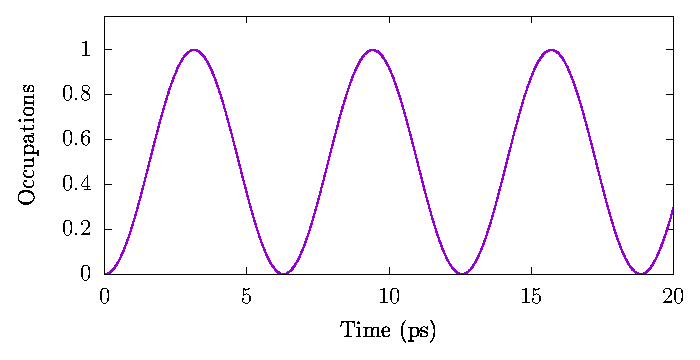
\includegraphics[width=20cm]{figs/example1.eps}
%\caption{\label{fig:rabi}
%Test.}
%\end{figure}

The same result can be obtained creating and editing the file 
\texttt{driver1.param}:


\noindent\makebox[5cm]{\rule{7cm}{0.4pt}}
\begin{verbatim}
dt                   0.001 
te                  20 

add_Hamiltonian      {hbar/2*(|1><0|_2+|0><1|_2)}


outfile              ACE1.out
\end{verbatim}
\noindent\makebox[5cm]{\rule{7cm}{0.4pt}}

and running
\begin{verbatim}
> ACE -driver driver1.param
\end{verbatim}
or simply 
\begin{verbatim}
> ACE driver1.param
\end{verbatim}
I.e., the first parameter is interpreted as a driver file.

A more complicated scenario can be described by the 
following driver file (\verb+driver2.param+), where an initially excited 
TLS, optionally subject to radiative decay described by a 
Lindblad term, is driven by a Gaussian laser pulse:

\noindent\makebox[5cm]{\rule{7cm}{0.4pt}}
\begin{verbatim}
dt                   0.01
te                  20

initial             {|1><1|_2}

#add_Lindblad         0.5  {|0><1|_2}
add_Pulse            Gauss  10 1 1 0  {(|1><0|_2+|0><1|_2)}

outfile              ACE2.out
\end{verbatim}
\noindent\makebox[5cm]{\rule{7cm}{0.4pt}}

This produces the following dynamics:

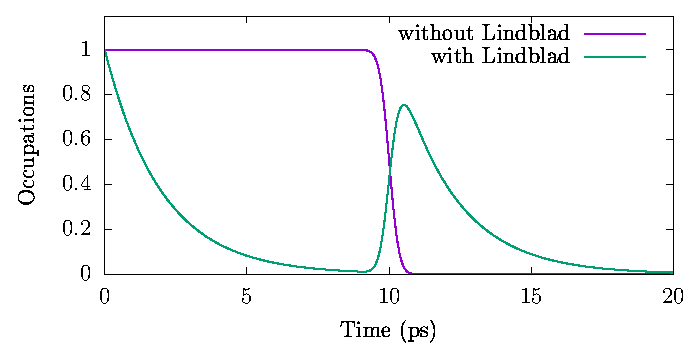
\includegraphics[width=20cm]{figs/example2.eps}

where the two curves are results of calculation where the Lindblad term is
either turned off or on. The \# symbol in a driver file indicates a comment, 
i.e. anything after it is ignored. The parameters of \texttt{add\_Lindblad}
are the rate $\gamma$ and the operator $A$ for the Lindblad term

\begin{equation}
\gamma \mathcal{L}[A](\rho)=\gamma\bigg[ A\rho A^\dagger 
-\tfrac 12\big(A^\dagger A\rho +\rho A^\dagger A \big)\bigg].
\end{equation}

The parameters of \verb+add_Pulse Gauss+ are the pulse center (here: 10 ps),
the pulse duration ($\tau_{FWHM}=1$ ps), the pulse area ($1 \pi$), the
detuning ($0$ meV), and the operator describing the light-matter coupling.

Finally, we mention that one can also explicitly specify which operator
average are to be printed into the output file by the parameter 
\verb+add_Output+, which takes as an argument an expression (in curly braces)
describing the respective operator. When it is first specified, the default
output operators are overridden and replaced by the specified operator average.
Specifying \verb+add_Output+ multiple times adds more columns to the output 
file.

\section{Environments}
In the following subsections, the usage of some of the predefined environments 
is demonstrated.
The driver files for the examples presented in the published article 
are contained in the first 4 subdirectories in the \texttt{examples} 
directory provided with the code.

\subsection{Fermionic environment}
One of the predefined 
environments is defined by the hopping Hamiltonian
\begin{equation}
H_E^k=\hbar g \big( c^\dagger_k c_S + c^\dagger_S c_k ) 
+ \hbar\omega_k c^\dagger_k c_k
\end{equation}
Here, the system is meant to be a Fermionic state that may be occupied or not.
The occupation is created by $c^\dagger_S$ or destroyed by $c_S$. 
Similarly, the environment consists of several Fermionic states, whose 
occupations are created and destroyed by $c^\dagger_k$ and $c_k$, respectively.
In the limit $N_E\to \infty$, the environment consists of a continuum of state,
which can be used to model the electronic states in metallic leads in
proximity to a quantum dot.
Consider the driver file:

\noindent\makebox[5cm]{\rule{7cm}{0.4pt}}
\begin{verbatim}
te                  5
dt                  1e-2
threshold           1e-7

Leads_N_modes       2
Leads_g             1 
Leads_omega_min     0
Leads_omega_max     0
Leads_EFermi        1e4

outfile             ACE3.out
\end{verbatim}
\noindent\makebox[5cm]{\rule{7cm}{0.4pt}}

Whenever we add an environment, we should specify a compression 
\verb+threshold+ (denoted $\epsilon$ in the paper). The smaller the
threshold, the more accurate the simulation. 
However, for very smaller thresholds also the calculation times as well as
the memory demands increase.

\verb+Leads_*+ indicates that what comes after is a parameter for
the leads-type environment specified by the above Hamiltonian. 
\verb+Leads_N_modes+ tells the code to use 2 Fermionic states as environment.
The coupling strength is determined by \verb+Leads_g+ and the energies 
are equidistantly sampled from \verb+Leads_omega_min+ to \verb+Leads_omega_max+
(in picoseconds; there also exist \verb+Leads_E_min+ and \verb+Leads_E_max+ 
if we want to specify the band width in units of meV).
Here, both limits are set to zero, so that both environment modes are 
resonant to the TLS transition. By setting \verb+Leads_EFermi 1e4+ (note that
1e4 is the C++ notation for $1\times 10^4$) the Fermi level is set to such
a high value that all environment states are initially occupied. 
There is also the parameter \verb+Leads_temperature+ to specify the temperature
(in units of Kelvin) of the Fermi distribution. 
If not specified, the global \verb+temperature+ 
parameter will be used, whose default is 4 K.
The initial state of the system is empty. Therefore, electrons will 
start to move from the leads to the system.
The dynamics is show below and it is discussed further in the article.

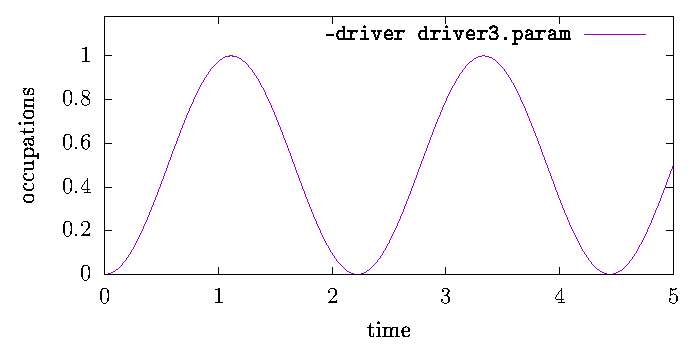
\includegraphics[width=20cm]{figs/plot_hopping_N2.eps}


Typically, the environments of open quantum system are assumed to form 
a continuum. In ACE, we simply discretize the continuum. For the case 
of metallic leads, it turns out that using $N_E=10$ modes is already
not too bad. 
Consider the driver file \verb+driver4.param+:

\noindent\makebox[5cm]{\rule{7cm}{0.4pt}}
\begin{verbatim}
te                  2.5
dt                  1e-2
threshold           1e-7

Leads_N_modes      10
Leads_rate          1 
Leads_omega_min    -5
Leads_omega_max     5
Leads_EFermi        1e4

outfile             ACE4.out
\end{verbatim}
\noindent\makebox[5cm]{\rule{7cm}{0.4pt}}

Here, instead of \verb+Leads_g+, we use \verb+Leads_rate+ to specify the 
rate that we would expect in the Markov limit. Then, the coupling constant  
is calculated internally by solving the Fermi's golden rule expression for $g$.
The respective dynamics is compared with the Markovian result
$1-\exp(-x)$ in the following plot:

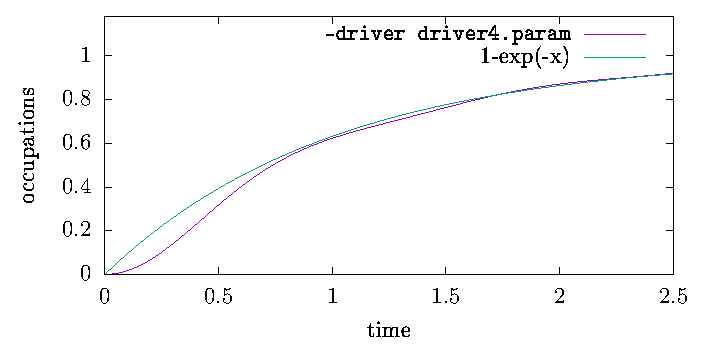
\includegraphics[width=20cm]{figs/plot_hopping_N10.eps}

Increasing $N_E$ even further to about 100 while keeping the same density of 
states (i.e. increasing the band width simultaneously) will produce a behaviour
very close to the Markovian results.

\subsection{Radiative decay}
The coupling of a quantum emitter to the electromagnetic field modes of free
space gives rise to radative decay and can be described by the Hamiltonian
\begin{equation}
H=\sum_{\mathbf{k}} \bigg[\hbar\omega_\mathbf{k}a^\dagger_\mathbf{k}a_\mathbf{k}
+ \hbar g_\mathbf{k}\big(a^\dagger_\mathbf{k} |G\rangle\langle X|
+a_\mathbf{k} | X\rangle\langle G| \big) \bigg],
\end{equation}
where $a^\dagger_{\mathbf{k}}$ and $a_{\mathbf{k}}$ are Bosonic creation and
annihilation operators. In practice, $\mathbf{k}$ is a three-dimensional
vector and the photon bands $\mathbf{k}$ may be modified by structuring the
photon environment, e.g. by embedding the emitter in a microcavity. 

%
Here, we assume isotropy (i.e., we work exclusively with the modulus 
$k=|\mathbf{k}|$) and a flat spectral density of state (as a function of 
the modulus $|\mathbf{k}|$), and discretize the light field continuum 
equidistantly. 
The only difference between this situation and the coupling
to Fermionic leads is that the mode operators are Bosonic, i.e., they can
in principle contain an arbitarily large number of excitations and the 
initial state is given by a Bose distribution instead of a Fermi distribution.
Therefore, we use the same set of parameters, just replacing 
\verb+Leads_*+ by \verb+RadiativeDecay_*+. Additionally, we use
the parameter \verb+RadiativeDecay_M+ to specify the cut-off in the number
of excitations (dimension of the respective Hilbert space, i.e., 1+maximal 
number of photons per mode; default value: 2).

\subsection{Phonons/spin-boson model/independent-boson model}
A TLS diagonally coupled to a continuum of independent bosons is known
as the independent-boson model or spin-boson model.
It also describes the coupling between a quantum dot (QD) and longitudinal
acoustic phonons. In this example, we take the latter as our use case.
The corresponding Hamiltonian is

\begin{equation}
H_E=\sum_{\mathbf{q}}\bigg[
\hbar\omega_{\mathbf{q}} b^\dagger_{\mathbf{q}}b_{\mathbf{q}}+
\hbar\gamma_{\mathbf{q}} \big( b^\dagger_{\mathbf{q}}+b_{\mathbf{q}}\big)
|X\rangle\langle X|\bigg],
\end{equation}

where $b^\dagger_{\mathbf{q}}$ and $b_{\mathbf{q}}$ are creation and
annihilation operators for phonons with wave vector $\mathbf{q}$.
It can be shown that the effects of such an environment are fully
characterized by the spectral density

\begin{equation}
J(\omega)=\sum_{\mathbf{q}} 
\gamma^2_{\mathbf{q}} \delta(\omega-\omega_{\mathbf{q}})
\end{equation}

Solving the original Hamiltonian is very difficult when the number of
phonon modes is large. Thus, we instead solve a replacement Hamiltonian 
by discretizing the respective spectral density $J(\omega)$. 
Internally, we can specify arbitrary spectral densities. However, so far only
the spectral density for phonons (described in the article) is accessible
via command line options.
A working driver file may be:

\begin{verbatim}
QDPhonon_temperature           4         # default: 4

QDPhonon_subtract_polaron_shift  true    # default: true   
QDPhonon_N_modes    100          
QDPhonon_M_max        3                  # default: 4
QDPhonon_E_max        5                  # default: 4
\end{verbatim}

Here, \verb+QDPhonon_N_modes+ is the number of modes, i.e. the 
number of sample points for the discretization.
\verb+QDPhonon_E_max+ is the cut-off energy determining the maximal 
value of $\omega$ for the discretization of $J(\omega)$. 
\verb+QDPhonon_M_max+ is the dimension of the Hilbert space for a single 
phonon mode (1+maximal number of phonons per mode). 
The temperature for the initial state of the bath is given by
\verb+QDPhonon_temperature+ (if not specified, \verb+temperature+ is checked).
By setting \verb+QDPhonon_subtract_polaron_shift+ to \verb+true+ (which is
the default behaviour) the polaron shift 
$-\sum_{\mathbf{q}}(\gamma^2_{\mathbf{q}})/(\omega_{\mathbf{q}})$ 
is subtracted from (i.e. the modulus is added to) the Hamiltonian. 
This is done to eliminate the effects of the polaron shift when comparing
calculations with and without phonons, which would otherwise affect 
resonance conditions.


As an alternative to ACE, the process tensor for Gaussian baths can be 
calculated using expressions where the bath is already integrated out
[cf. {J{\o}rgensen and Pollock} Phys. Rev. Lett. 123, 240602 (2019)]. 
This method is usually much more 
efficient and does not require discretization or truncation of the phonon
Hilbert spaces (Recall: The advantage of ACE is its generality, while 
the latter method only works for Gaussian baths.)
To use this method instead for phonon simulations with our standard 
phonon spectral density, the following can be added to the driver file:

\begin{verbatim}
use_process_tensor     true
temperature            4
\end{verbatim}


\iffalse
\subsection{Spins}

\begin{equation}
H=\sum_k J_k \mathbf{S}\cdot \mathbf{s}_k 
\end{equation}

\begin{verbatim}
#RandomSpin_set_initial_dir 0 0 1
#RandomSpin_B_eff    0 0 0 

RandomSpin_B_init      0 0 1
RandomSpin_T           4

RandomSpin_N_modes         10
RandomSpin_J_max            0.1
RandomSpin_J_min            0.1
RandomSpin_seed             1

RandomSpin_print_initial    RandomSpin_T4_B1_normJ_N10_te20_dt1e-2_thr1e-10.init
\end{verbatim}

\subsection{Combining process tensors}

\fi

\section{Concluding remarks}
Further developments of ACE as well as the code are ongoing projects.
The documentation naturally lags behind. 

\end{document}
